% %%%%%%%% ICML 2025 WORKSHOP EXTENDED ABSTRACT SKELET ON %%%%%%%%%%%%%%%%%
% % Based on the main ICML 2025 template
\documentclass[twocolumn]{openjournal}

\usepackage{hyperref}
\hypersetup{
    colorlinks=true,
    linkcolor=blue,
    filecolor=blue,      
    urlcolor=gray,
    citecolor=blue,
}
\usepackage{arydshln}
\usepackage{xcolor}
\usepackage{textgreek}
\usepackage[utf8]{inputenc}
\usepackage[english]{babel}


\usepackage{color,colortbl}
\usepackage{tensind}
\tensordelimiter{?}
\DeclareGraphicsExtensions{.bmp,.png,.jpg,.pdf}
\usepackage{graphicx}

\usepackage{subcaption}
\let\longtable\undefined
\usepackage{verbatim}
\usepackage[normalem]{ulem}
\usepackage{orcidlink}
\usepackage{soul}
\usepackage{bm}
\urlstyle{same}
\usepackage{amsmath}
\usepackage{float}
\usepackage{color}
\usepackage{xcolor}
\usepackage{booktabs}
\usepackage{cleveref}
% In your preamble, make sure you have these packages:
% \let\longtable\undefined

\begin{document}

\title{Nested Sampling for Future Inference: GPU-NS and Emulation for feasible evidence calculation on high-dimensional likelihoods}

\author{}

\email{lovicktoby@gmail.com}
\affiliation{Institute of Astronomy, University of Cambridge, Cambridge, UK}

\begin{abstract}
We demonstrate a GPU-accelerated nested sampling framework for efficient high-dimensional Bayesian inference in cosmology. Using emulators and JAX-based calculations for rapid likelihood evaluations of Cosmic Microwave Background (CMB) and the matter power spectrum for a cosmic shear analysis, our approach provides parameter constraints and direct calculation of Bayesian evidence. Where CPU-based nested sampling can now be outpaced by methods relying on MCMC sampling and decoupled evidence estimation, we demonstrate that with GPU acceleration nested sampling offers the necessary speed-up to put it on equal computational footing with these methods, especially where reliable model comparison is paramount.
\end{abstract}

\section{Introduction}  
\label{sec:introduction}
Bayesian inference offers a principled statistical framework for parameter estimation and model comparison, and is widely employed in astrophysics for distinguishing between competing cosmological theories \citep{Trotta_2008}. The advent of large-scale surveys such as Euclid \citep{euclid}, the Vera C. Rubin Observatory \citep{Vera}, and the Nancy Grace Roman Space Telescope \citep{nancy}, alongside increasingly sophisticated theoretical models, has led to a significant increase in both data volume and model dimensionality. While maximum likelihood values and parameter estimation remain manageable in this new scale of problem, the accurate computation of the Bayesian evidence stands as a distinct computational hurdle. Bayesian evidence is very valuable as a model comparison tool, as it weighs goodness of fit against model complexity, naturally penalizing over-fit models \citep{Lovick:2023tnv}.

To address these high-dimensional inference challenges, the field has undergone significant algorithmic innovation. Advanced Markov Chain Monte Carlo (MCMC) techniques, including gradient-based samplers like Hamiltonian Monte Carlo (HMC) and No-U-Turn Sampler (NUTS) which utilise differentiability for efficiency \citep{jaxcosmo, Dupourqu__2024}, Variational Inference (VI) offering an optimization-based alternative \citep{VIacceleration}, and machine learning-augmented approaches, such as neural emulators for rapid likelihood approximation \citep{Piras_2023} and the learned harmonic mean estimator for decoupled Bayesian evidence estimation \citep{Piras_2024,polanska2025learnedharmonicmeanestimation}, have emerged as promising methods. Concurrently, the parallel processing capabilities of Graphics Processing Units (GPUs) have been identified as an important development, accelerating likelihood evaluations and sample generation across diverse methodologies \citep{Gu_2022, GPUacc,metha}, and extending the scope of feasible analyses.

Nested Sampling (NS) \citep{Skilling06} is a notable meta-algorithm that offers simultaneous parameter inference and direct Bayesian evidence calculation from a single execution, a key advantage for rigorous model selection, while also effectively exploring complex, multimodal posterior landscapes. Although traditional CPU-based NS implementations have encountered scalability limitations in high-dimensional settings, recent work to adapt Nested Sampling to efficiently utilize GPU-hardware \citep{NSSyallup} has pushed the capabilities of the algorithm much further than its CPU counterpart. Our work demonstrates that GPU-accelerated Nested Sampling is significantly faster than its CPU counterparts on a pair of cosmological likelihoods, and that it serves as a competitive and robust method for Bayesian inference in astrophysics and cosmology.

\section{Methodology}
\label{sec:methodology}
\subsection{Nested Slice Sampling}
For a full review of Nested Sampling aimed at physical scientists, see \citep{Ashton_2022}. Nested sampling is a Monte Carlo method designed to draw posterior samples and calculate the Bayesian evidence, $\mathcal{Z}$, defined as the integral of the likelihood $\mathcal{L}$ over the prior distribution $\pi$ of the parameters $\theta$:
\begin{equation}
    \mathcal{Z}=\int \mathcal{L}(\theta) \pi(\theta) d\theta. \label{eq:evidence}
\end{equation}
The algorithm iteratively replaces the point with the lowest likelihood among a set of ``live point'' with a new point drawn from the prior, constrained to have a likelihood higher than the point being replaced. This process allows the evidence to be accumulated as a sum of likelihood values weighted by successively smaller prior volumes. Nested Sampling is well established as one of the primary methods for estimating the Bayesian evidence of models in cosmology, appearing in many contemporary high profile results~\citep{planck,DES:2021wwk}.

The key challenge of implementing NS is to efficiently draw samples from the prior within these progressively shrinking, hard likelihood boundaries. Slice sampling~\citep{neal_slice_2003} is an MCMC technique well-suited for this task, as it can adaptively sample from such constrained distributions without requiring manual tuning of proposal scales. Usage of slice sampling within nested sampling was popularised in \cite{polychord}. Slice sampling works by sampling uniformly from an auxiliary variable defining a ``slice'' under the likelihood surface and then sampling the parameters from the region within that slice. The work of \cite{NSSyallup} provided a generic implementation of the nested sampling algorithm, as well as a tailored implementation of a slice sampling based algorithm that was designed specifically to be amenable to the massive parallelism opportunities of modern GPUs. The latter implementation is styled as \emph{Nested Slice Sampling} (NSS), and we adopt this specific algorithm in this work.

\subsection{Sampler Parallelisation}\label{samplerparall}

Nested sampling can be parallelised by selecting the $n$  live points with the lowest likelihoods rather than just the lowest, and evolving them with the likelihood constraint in parallel. This adaptation does not introduce new approximations into the core NS algorithm itself; rather, it significantly enhances computational speed by harnessing parallel hardware capabilities. If the generation of new points can be vectorized or batched, this represents a substantial potential speed-up for GPU execution, and evolving many points at once should scale as $\mathcal{O}(1)$ with the number of points, up to the parallelisation limit of the GPU.

The primary computational bottleneck in this parallel scheme becomes the speed of bulk likelihood evaluations. This necessitates the use of JAX-based likelihoods and emulation in place of traditional Boltzmann codes, such as those provided by \texttt{cosmopower-jax} \citep{Piras_2023}, to fully utilise the GPU's parallel processing power for these evaluations. The NSS implementation is provided in the \texttt{blackjax}~\citep{cabezas_blackjax_2024} framework. As a native \texttt{jax}~\citep{deepmind_deepmind_2020} \emph{compilable} sampling framework, this is well positioned to exploit the parallelisation opportunites present at the likelihood level, reducing key factors such as communication overhead between devices that can plague hardware accelerated workflows.

In contrast, MCMC-based methods can access GPU vectorization by running multiple independent chains in parallel. The generation of a new sample within a single chain is an inherently sequential process, so its speed is limited by the evaluation time of the likelihood function. While running many chains in parallel is an effective use of the GPU, this strategy requires that each chain independently reaches convergence, so the need for a ``burn-in" period for each chain to discard its initial non-stationary samples \citep{hoffman14a} means that the efficiency does not scale as directly as batching an NS run.

% DY: I believe the below should be rewritten s.t. harmonic is the "afterburner" for estimating evidences and HMC (NUTS)? is the sampling algorithm. I would move all mention of harmonic to a paragraph after this along the lines: "As the target of this analysis is ultimately the Evidence, we employ the harmonic framework on the HMC samples acquired as described above...". Depending on detail of HMC algorithm may wish to mention~\citep{hoffman_tuning-free_2022,hoffman_adaptive-mcmc_2021} targetting tuning of HMC on massively parallel devices.
For our HMC comparison, we employ the \texttt{harmonic} framework \citep{mcewen2023machinelearningassistedbayesian}, which trains a normalizing flow on posterior samples in order to compute the evidence via the learned harmonic mean estimator. The evidence values reported in Table \ref{tab:results} utilize the same flow architecture and training procedure as in \citep{Piras_2024}, although other architectures are explored in Section \ref{flowscatter}. We found that for the Cosmic Shear likelihood, a reparametrisation of the Gaussian nuisance parameters was necessary to achieve efficient sampling \citep{Betancourt2017HMC}. Without this transformation, the HMC sampler required approximately four times the computation time and produced a high rate of divergences, rendering the output unsuitable for inference. In this work \texttt{polychord} \citep{polychord,Polychord2} provides the comparison for a CPU-based nested sampler.

\subsection*{CMB and Cosmic Shear Analyses}
We demonstrate the sampler on a pair of cosmological problems: a cosmic variance-limited CMB power spectrum analysis and a Cosmic Shear analysis. The CMB analysis, a standard 6-dimensional problem, functions as a benchmark and demonstration of the sampler's speed when used on a highly vectorisable likelihood, and its accuracy on a foundational application \citep{planck}. The Cosmic Shear analysis, with 7 cosmological and 30 nuisance parameters, presents a higher dimensional challenge that represents the edge of what CPU-based nested sampling can manage, and offers a direct comparison to the HMC + learned Harmonic Mean Estimator analysis of \cite{Piras_2024}.
\begin{figure*}[ht]
    \centering % Center the entire figure content
    % --- Left Subfigure: CMB Scaling ---
    \begin{subfigure}[b]{0.48\textwidth}
        \centering
        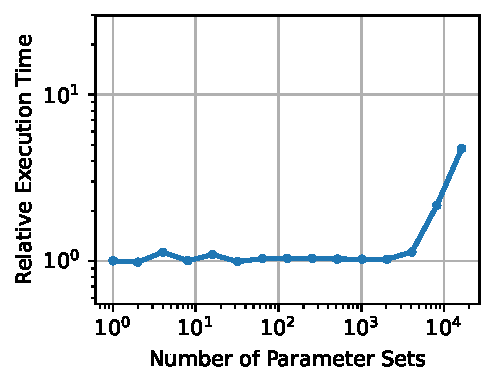
\includegraphics{cmbscaling.pdf}
        \caption{CMB Likelihood as timed on an L4 GPU, with near-perfect vectorization up to $\mathcal{O}(10^3)$ parallel calls}
        \label{fig:cmb_scaling}
    \end{subfigure}
    \hfill % This command adds horizontal space to push the figures apart
    % --- Right Subfigure: Cosmic Shear Scaling ---
    \begin{subfigure}[b]{0.48\textwidth}
        \centering
        % IMPORTANT: Replace 'Shear_scaling.pdf' with the actual filename 
        % for your plot showing both interpolated and full scaling.
        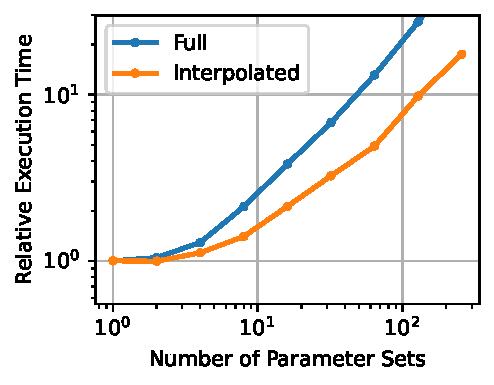
\includegraphics{shearscaling.pdf} 
        \caption{Shear Likelihood timed on an A100 GPU, where using interpolation introduces some vectorisation}
        \label{fig:shear_scaling}
    \end{subfigure}
    % --- Main Figure Caption ---
    \caption{Execution time for batched likelihood evaluations for both the CMB and Cosmic Shear likelihoods.}
    \label{fig:likelihood_scaling}
\end{figure*}
\subsection{CMB TT Power Spectrum}
The CMB TT power spectrum analysis is kept deliberately simple by assuming a cosmic variance-limited scenario. In this idealized case, the uncertainty in the power spectrum measurements $C_\ell^{\text{obs}}$ at each multipole $\ell$ is due only to the inherent statistical fluctuations of the CMB itself, rather than instrumental noise or foreground effects. The likelihood for the observed power spectrum, given a theoretical model $C_\ell(\theta)$ follows a chi-squared distribution of shape $2\ell +1$ \citep{planck}. The \texttt{cosmopower-jax} emulator suite provides the predictions for $C^{TT}_\ell(\theta)$, allowing them to be vectorized very efficiently. This likelihood is run on mock data generated from the Planck best-fit parameters \citep{planck}.

\subsection{Cosmic Shear}
We use the likelihood framework described in \citep{Piras_2023,Piras_2024}. Cosmic shear refers to the weak gravitational lensing effect where the observed shapes of distant galaxies are coherently distorted by the intervening large-scale structure of the Universe \citep{Kilbinger_2015}. This distortion is quantified by the angular shear power spectra $C_\ell^{\kappa\kappa}$.

The theoretical prediction for these $C_\ell^{\kappa\kappa}$ values involves integrating over the matter power spectrum $P(k,z)$ and the lensing efficiency, which depends on the redshift distribution of source galaxies. \texttt{cosmopower-jax} is used to emulate the linear and non-linear matter power spectrum, and the $C_\ell^{\kappa\kappa}$ are calculated using the extended Limber approximation \citep{LoVerde_2008}, which translates between Fourier modes $k$ and multipoles $\ell$. The likelihood for observed shear power spectra $C_\ell^{\text{obs}}$ given a model $C_\ell^{\text{th}}(\theta)$ is assumed to be a multivariate Gaussian, again run on mock data.

We closely follow the methodology of the \texttt{cosmopower-jax} implementation papers \citep{Piras_2023}. We consider a tomographic survey with $N_{\text{bins}}=10$ redshift bins. The primary observable is the set of angular power spectra $C^{\epsilon \epsilon}_{i j} (\ell)$ between all pairs of bins $(i,j)$. This signal is composed of the true cosmic shear signal ($\gamma$) and a significant contaminant from the intrinsic alignments ($I$) of galaxies:
\begin{equation}
	C^{\epsilon \epsilon}_{i j} (\ell) = C^{\gamma \gamma}_{i j} (\ell) + C^{\gamma I}_{i j} (\ell) + C^{I \gamma}_{i j} (\ell) + C^{I I}_{i j} (\ell).
\end{equation}
Each of these components is computed using the extended Limber approximation \citep{LoVerde_2008}, which projects the 3D matter power spectrum, $P_{\delta \delta}(k,z)$, into a 2D angular correlation:
\begin{equation}
	C^{A B}_{i j} (\ell) = \int_0^{\chi_H} \frac{W_i^A (\chi)  W_j^B (\chi)}{\chi^2}  P_{\delta \delta} \left(k = \frac{\ell + 1/2}{\chi}, z \right) \mathrm{d}\chi,
\end{equation}
where $\{A, B\} \in \{\gamma, I \}$, $\chi$ is the comoving distance up to the horizon $\chi_H$, and $W(\chi)$ are the window functions for each component.

The shear window function $W^\gamma(\chi)$ depends on the underlying cosmology and the redshift distribution $n_i(z)$ of source galaxies in each tomographic bin $i$:
\begin{equation}
	W_i^\gamma (\chi) = \frac{3 \Omega_{\rm m} H_0^2 }{2  c^2} \frac{\chi}{a(\chi)} \int_{\chi}^{\chi_{\rm H}}   n_{i}(\chi')  \frac{\chi'-\chi}{\chi'} \mathrm{d} \chi'.
\end{equation}

\textbf{Nuisance Parameters:} To achieve the precision required by modern surveys, we must also model several systematic effects, each of which introduces nuisance parameters that must be marginalized over.
\begin{itemize}
    \item \textbf{Intrinsic Alignments ($A_{\text{IA},i}$):} The intrinsic shapes of nearby galaxies can be physically correlated, mimicking a lensing signal. We model this using the Non-Linear Alignment (NLA) model \citep{hirata_04} as parametrised in \citep{Piras_2023}, which defines the intrinsic alignment window function $W^I$. We introduce a single free amplitude parameter per bin, $A_{\text{IA},i}$, controlling the strength of the signal:
    \begin{equation}
    	W_i^{\rm I}(\chi) = - A_{\mathrm{IA}, i}  \frac{C_1  \rho_{\rm cr}  \Omega_{\rm m}}{D(\chi)}  n_{i}(\chi),
    \end{equation}  
     which is sensitive to the linear growth factor $D(\chi)$, the critical density of the universe $\rho_{\rm cr}$, and a normalization constant $C_1$ fixed to $5 \times 10^{-14} \, h^{-2} M_\odot^{-1} \text{Mpc}^3$.     This adds 10 nuisance parameters to our model.
    \item \textbf{Multiplicative Shear Bias ($m_i$):} Imperfections in the shape measurement algorithms can lead to a systematic bias in the measured shear, which we model with a multiplicative factor $m_i$ for each bin. The observed shear spectrum is rescaled by $(1 + m_i)(1 + m_j)$. This introduces another 10 nuisance parameters.

    \item \textbf{Photometric Redshift Errors ($D_{z_i}$):} Uncertainties in photometric redshift estimation can shift galaxies between bins. We model this with a simple shift parameter $D_{z_i}$ for the mean of each redshift distribution, $n_i(z) \rightarrow n_i(z - D_{z_i})$, adding a final 10 nuisance parameters.
\end{itemize}

This results in a pair of models with 7/9 cosmological parameters ($\Omega_m, \Omega_b, h, n_s, \sigma_8, \Omega_k, w_0, w_a$) and 30 nuisance parameters ($\{A_{\text{IA},i},m_i,D_{z_i}\}$), for a total of 37/39 dimensions. The likelihood for the data vector of all $C_\ell$s is assumed to be a multivariate Gaussian, with a simulated covariance matrix for an LSST-like survey ($n_{\text{gal}} = 30\,\text{arcmin}^{-2}$, $\sigma_{\epsilon} = 0.3$, $f_\text{sky} = 0.35$). The complexity and dimensionality of this forward model highlight the need for the GPU-accelerated framework developed in \cite{NSSyallup} and showcased here.
\begin{table*}[ht]
\caption{The Evidence and computation times for the models and samplers considered. Computation times are the time taken to run both cosmologies, and are compared qualitatively. Shown also are the times reported by \cite{Piras_2024} (denoted by \textbf{*}) for comparison.}
\label{tab:results} 
\vskip 0.15in
\begin{center}
\begin{small}
\begin{tabular}{llcc|c|crr}
\toprule
Model  & Method & $\log \mathcal{Z}_{\Lambda\text{CDM}}$ & $\log \mathcal{Z}_{w_0w_a}$ & $\log B_{01}$ & Computation Time & Hardware \\ 
\midrule
CMB  &  \texttt{polychord} & 87573.4$\pm$ 0.3&  &&  $\sim$1 hour  & 1 CPU \\
  &  NS & 87573.6$\pm$ 0.3&  & & $\sim$12 seconds  & 1 L4 GPU \\
 &  NUTS + harmonic & 87572.3$\pm$ 0.0076& & &  $\sim$2 minutes  & 1 L4 GPU \\
\midrule
Cosmic Shear  & NS (Interpolation) &  $40959.03 \pm 0.31$ & $40956.28 \pm 0.32$ & $2.74 \pm 0.44$ & $\sim$11 hours  & 1 A100 GPU &  \\
 &   NS (Full) &  $40958.09 \pm 0.31$ & $40955.49 \pm 0.33$ &$ 2.60 \pm 0.47$& $\sim$2 Days  & 1 A100 GPU &  \\
    &  HMC (Interpolation) & $40956.67\pm  0.38$ &  $40954.05 \pm 0.39 $& $2.62 \pm 0.55 $ & $\sim$6 Hours & 1 A100 GPU  \\ \midrule
Cosmic Shear*   &  \texttt{polychord} & $-107.03\pm 0.27$& $-107.81 \pm 0.74$& $0.78 \pm 0.79$& $\sim$8 Months  & 48 CPUs \\
   &  HMC (Full) & $40956.55 \pm 0.06$& $40955.03 \pm 0.04$ & $1.53 \pm 0.07$ & $\sim$2 Days &12 A100 GPUs \\ 

\bottomrule
\end{tabular}
\end{small}
\end{center}
\vskip -0.1in
\end{table*}
To fully leverage the vectorization capabilities of JAX, significant modifications were made to the original likelihood code. The original implementation, built around `cosmology' class objects, offers high interpretability but is not amenable to JAX's just-in-time (JIT) compilation of pure functions. We therefore refactored the likelihood into a series of stateless functions. This process resulted in a less general but highly optimized code path. Extensive validation was performed to ensure consistency between the two versions, with minor (sub 0.1\%) numerical differences owing to slightly different choices of $\chi, D(\chi)$ implementations. By re-running HMC on our optimised likelihood we isolate the performance of each sampling method on the same likelihood function.

As shown in figure \ref{fig:shear_scaling}, the full Cosmic Shear likelihood calculation is compute-intensive and does not scale efficiently beyond a small number of parallel evaluations. To mitigate this bottleneck, we implemented an alternative version of the likelihood where the matter power spectrum emulator is evaluated over a smaller $z$-grid and interpolated. This trades accuracy for computational throughput and offers a comparison to the performance of a less computationally intensive likelihood. "e report these results as the "Full" and "Interpolated" likelihoods. The same interpolated likelihood was used for the HMC comparison.

The prior ranges for each parameter are given in table \ref{tab:shearpriors}

\begin{table}[h!]
\centering
\caption{Prior distributions for the model parameters, split into cosmological, Baryonic, and nuisance parameters.}
\label{tab:shearpriors}
\begin{tabular}{c c}
\toprule
\textbf{Parameter} & \textbf{Prior Range} \\
\midrule

$\omega_b = \Omega_b h^2$ & $\mathcal{U}(0.01875, 0.02625)$ \\
$\omega_\text{cdm} = \Omega_\text{cdm} h^2$ &  $\mathcal{U}(0.05, 0.255)$ \\
$h$ &  $\mathcal{U}(0.64, 0.982)$ \\
$n_s$ & $\mathcal{U}(0.84, 1.1)$ \\
$\ln 10^{10}A_s$ & $\mathcal{U}(1.61, 3.91)$ \\
$w_0$ &  $\mathcal{U}(-1.5, -0.5)$ \\
$w_a$ &  $\mathcal{U}(-0.5, 0.5)$ \\
\midrule
$c_\text{min}$ & $\mathcal{U}(2, 4)$ \\
$\eta_0$ & $\mathcal{U}(0.5, 1)$ \\

\midrule

$A_{\text{IA},i}$  & $\mathcal{U}(-6, 6)$ \\
$D_{z_i}$ & $\mathcal{N}(0, 0.01^2)$ \\
$m_i$   & $\mathcal{N}(0.01, 0.02)$ \\
\bottomrule
\end{tabular}
\end{table}

\section{Results}
\label{sec:results}
We present the results of our comparative analyses in Table \ref{tab:results}, detailing the Bayesian evidence values and computation times for both the CMB and Cosmic Shear problems. For each problem, we compare our GPU-accelerated Nested Sampler (GPU-NS) against a traditional CPU-based NS implementation (\texttt{polychord}) and a modern HMC sampler coupled with a learned harmonic mean estimator (\texttt{harmonic}). We ran the GPU-NS with 1000 live points in both cases, and for HMC we ran 60 chains with 100/400 warm-up/samples and 400/2000 for the CMB and shear likelihoods respectively. For the shear likelihood these numbers were chosen to match the sampling strategy of \cite{Piras_2024}, and for the CMB the total number of samples was scaled down for the dimension of the problem, in line with the decrease in nested samples taken. 

\subsection{CMB results}
% \begin{figure}[b]
%     \centering
%     \includegraphics[width=0.9\linewidth]{computation_times.pdf}
%     \caption{The total computation time required to calculate the Bayesian evidence for $\Lambda$CDM and $w_0w_a$ for both HMC and NSS, with and without interpolation. HMC was only run with interpolation to provide a comparison, and the projection here is based on the performance of NSS.}
%     \label{timings}
% \end{figure}
The CMB analysis highlights the ideal use-case for GPU-NS. As shown in \cref{fig:cmb_scaling}, the emulator-based likelihood is highly vectorisable, and so our GPU-NS approach completes the analysis in just 12 seconds, a speed-up of nearly 300x compared to the 1 hour required by the CPU-based \texttt{polychord}. While \texttt{polychord} updates a single live point per iteration, our method evolves 500 live points in parallel, fully exploiting the GPU's architecture. This performance gain would be even more pronounced against traditional, non-emulated likelihoods based on codes like CAMB, which are significantly slower per evaluation.

The comparison with HMC in this regime is very instructive. While HMC is also fast, taking only $\sim2$ minutes, it does not match the raw speed of GPU-NS. This is because the primary advantage of HMC; its ability to take large, efficient steps using gradient information, isn't as impactful as being able to vectorise the sampling en-masse. In this scenario, the parallelisation efficiency of the NS algorithm allows it to brute-force the calculation more rapidly than the multi-chain HMC approach.

\subsection{Cosmic Shear Results}
We find great success in the 37/39-dimensional Cosmic Shear analysis where our GPU-NS framework transforms an analysis that is practically infeasible with CPU-based NS ($\sim$8 months reported in \citep{Piras_2024}) into a task that can be completed in approximately 2 days on a single A100 GPU. The cosmological posteriors are shown in figure \ref{shearmarg}, and the full 39-dimensional posterior is shown in the appendix. However in contrast to the massive parallelism of the CMB-only analysis, figure~\ref{fig:shear_scaling} demonstrates that the more computationally intensive shear likelihood inhibits the potential speed-up achievable on a single GPU.

An interesting finding of this work is the discovery of a secondary posterior mode in the Cosmic Shear likelihood, shown in the full posterior plot \ref{shearfull}. This mode, peaked around $A_{\text{IA},10} \sim 4.5$, was checked against the original \citep{jaxcosmo} likelihood, revealing that it is indeed a real missed mode. HMC found some small amplitude here, however due to the HMC sampler's sensitivity to its initialisation this peak was not correctly represented in the posterior samples.

\section{Discussion}

\begin{figure}
    \centering
    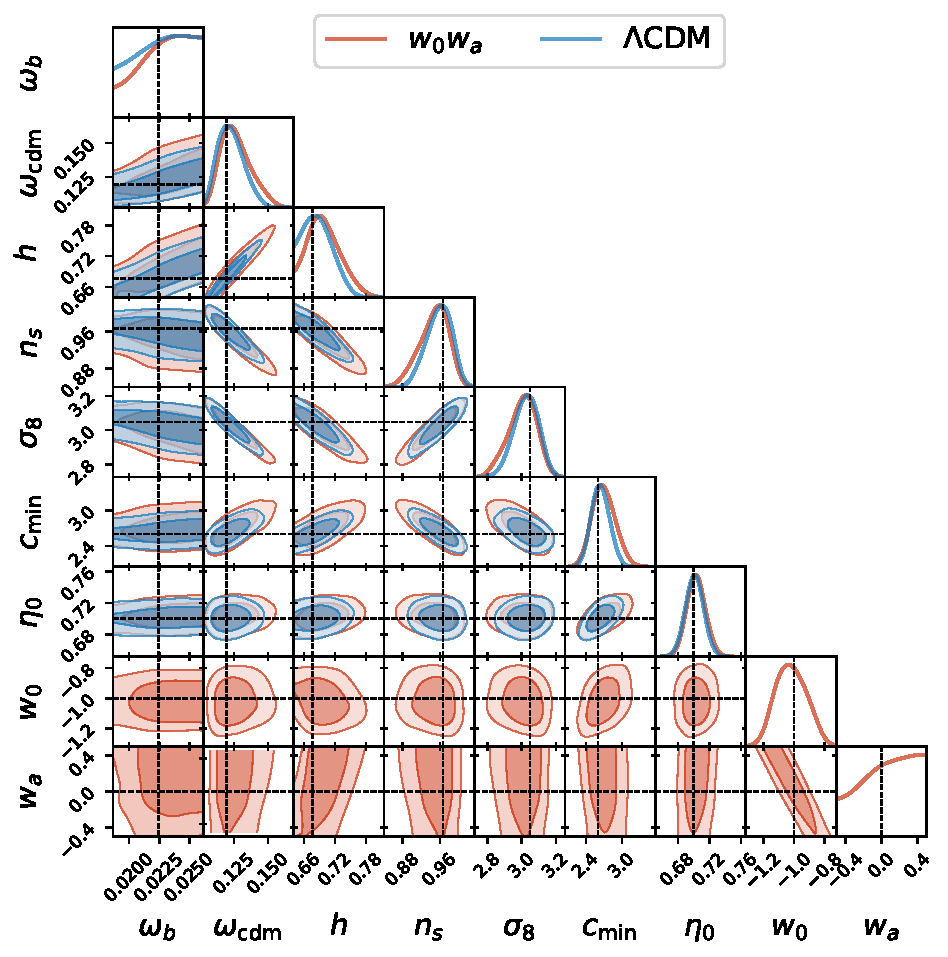
\includegraphics[width=0.9\linewidth]{w0wa_lcdm.pdf}
    \caption{Marginalized posterior distributions for the cosmological parameters of the Cosmic Shear analysis, using the full likelihoods with GPU-NS. The contours show the 68\% and 95\% credible intervals for each parameter}
    \label{shearmarg}
\end{figure}

\subsection{Performance Breakdown}
On the CMB likelihood, where as shown in figure \ref{fig:cmb_scaling} the likelihood perfectly vectorises well beyond our n\textunderscore live of 1000, nested sampling finds its biggest speed-up. As presented in \cite{NSSyallup}, the \texttt{blackjax} nested sampling implementation is a truly vectorised sampling procedure, and thus can fully leverage a vectorised likelihood. To make HMC approach this level of speed-up would require running 500 separate chains, and the scaling properties of the likelihood suggest that running this many chains would take no longer than running fewer chains. However, due to the need for a warm-up phase, as well as the auto-correlation that would be of concern when running chains that are too short, HMC cannot utilise a vectorised likelihood to the same degree, 500 chains of 20 samples does not have the same statistical power as 10 chains of 1000 samples.
%DY: this depends a bit on the flavour of HMC, optionally put the hoffman refs I listed earlier here as an example of "future work" that can incorporate more parallel friendly HMC
In the case that the likelihood is the bottleneck, such as in the shear likelihoods, GPU-NS loses its advantage, and the two algorithms sit on a fairly equal footing. Here all of the speed-up comes from the likelihood internally vectorising, so although the samplers cannot massively vectorise to speed up the inference, individual likelihood calls are greatly sped up by having their many internal emulator calls vectorised. The interpolated likelihood appears to benefit from being able to vectorise slightly more than the full likelihood, although it's speed-up is also consistent with the fact it makes less emulator calls per evaluation. 

There are a number of potential routes to lift this bottleneck further. All the calculations presented in this work are performed in double numeric precision, whilst it is non-trivial to ensure that sufficient accuracy in result is achievable with lower precision, it is noteworthy that much of the hardware development is targetting increasingly reduced numeric precision, and this is a development that physicists need to be alert to. Reducing the required numeric precision to single float numerics would greatly increase the potential to parallelise the calculations in this work. More immediately, it is also feasible to recover massive speedups by deploying the calculations over multiple devices/GPU clusters. The original work of ~\citep{Piras_2024} distributed it's MCMC chains over multiple devices, this enables faster (in wall-time) accumulation of multiple chains. However multiple chains in this context primarily improve the estimate of variance of the result, in contrast population level approaches such as NSS can improve total runtime (for a fixed variance) trivially using multiple devices.

%DY: a question from me, and more for future work. Surely the current explicit boltzmann solver (CAMB) based version of these analysis doesnt call CAMB 1000x for each likelihood? If the emulation is simple can we not be emulating something more directly that bypasses the need to call cosmopower 1000x for each likelihood? Perhaps we can motivate more targeted emulators as a route to lift the bottleneck here?

\subsection{Normalising Flow Hyperparameters}\label{flowscatter}
The evidence values quoted in table \ref{tab:results} are estimated using a normalising flow with 4 layers and a temperature of $\beta = 0.8$. However, motivated by the $\mathcal{O}(2)$ discrepancy between the NSS and HMC log-evidence values, we tested a range of normalising flow hyperparameters to see if a better fitting flow might provide a different evidence estimate.

We tried flows with temperatures ranging from 0.5 - 1.0, on both 2 and 4 layer normalising flows. The results of the estimator on each of these is shown in table \ref{tab:flow_sensitivity}. Each overall Bayes factor appears to be approximately equal, similarly to the comparison between the interpolated and full nested sampling evidences, but the evidence values from each flow do scatter decently beyond their reported error bars.

This demonstrates that some caution should be taken with the error bars provided by this estimator; it represents only the scatter in the estimate taken on different subsets of the data. It does not include any error from how the flow might change if trained on a different set of posterior samples, and most importantly there is no systematic error from the flow not capturing the true posterior shape. This incomplete error budget should be a serious concern, as presented the GPU-NS versus HMC results in table \ref{tab:results} are around $4\sigma$ away from each-other for the interpolated likelihood, and while each method appears to recover the same Bayes factor there is no guarantee this would be true in general, and a discrepancy of 2.5 in log space is the difference between decisive and inconclusive evidence when performing Bayesian model comparison.

%DY: I must confess I don't follow the arguments from a quick read of the harmonic paper as to how we can be using correlated samples here in the first place (i.e. no chain thinning) although this seems to be the recipe there and it gets reasonable results. I would have assumed there is a residual error that for a fixed calculation can only be estimated using leave one out cross validation or something of that ilk. I don't suggest we explore that here!
%DY: Whilst there are clear strengths of a decoupled model comparison approach, I do think this warrants careful demonstration that the ensemble chain settings are actually producing samples compatible with a long run - thinned - HMC chain, quoting metrics such as Rhat to demonstrate that we are actually mixing well.  

Nested Sampling, in turn, is not immune to its own implementation-specific biases, and its error bar is also conditional. The NS error calculation assumes that at each iteration, a new live point is drawn perfectly uniformly from the prior volume constrained by the current likelihood threshold \citep{Skilling06}. In practice, this is approximated with an inner MCMC sampler which, in high-dimensional or complex posteriors, can struggle to explore the entire valid region. This inefficiency can introduce a systematic bias that the reported statistical error does not account for. However, since nested sampling is a global algorithm, it does properly account for the error in the specific path taken when crossing from the prior to the posterior, and as a global algorithm it is unlikely to miss relevant modes when run at sufficient precision. Bringing the overall runtime of this challenging frontier problem to a level that multiple methods can be tested with rapid turn around is a significant success we highlight of the optimizations performed as part of this work. It is possible to investigate the discrepancy between the harmonic and NS based pipelines now by incorporating other advanced MCMC based normalizing constant estimators such as Sequential Monte Carlo~\citep{doucet_introduction_2001}. 

\begin{table}[t!]
\centering
\caption{Sensitivity of Bayesian evidence estimates to the normalizing flow temperature parameter $\beta$ and number of layers of the flow. A value of $\beta=1$ corresponds to the standard posterior, while lower values temper the distribution. All evidence values are derived from the learned harmonic mean estimator using flows trained at the specified $\beta$.}
\label{tab:flow_sensitivity}
\begin{tabular}{c c c c}
\toprule
\textbf{$\beta$} & \textbf{$\log \mathcal{Z}_{\Lambda\text{CDM}}$} & \textbf{$\log \mathcal{Z}_{w_0w_a}$} & \textbf{$\log B_{01}$} \\
\midrule
4 Layers \\
\midrule
0.50 & $40957.24 \pm 0.09$ &  & \\
0.6 & $40957.04 \pm 0.17$ &  & \\
0.7 & $40956.80 \pm 0.32$ & &  \\
0.8 & $40956.67 \pm 0.38$&& \\
0.9 & $40956.66 \pm 0.37$&& \\
1.0 & $40956.72 \pm 0.32$&&\\
\midrule 
2 Layers \\
\midrule
\bottomrule
\end{tabular}
\end{table}

\section{Conclusion}

We have demonstrated that the combination of GPU-acceleration, JAX-based emulators, and a vectorized Nested Sampling algorithm removes the primary computational barrier in using Nested Sampling in high-dimensional problems. Our framework achieves a speed-up of over two orders of magnitude on a cosmic-variance-only CMB analysis and, more critically, reduces the runtime of a 39-dimensional cosmic shear analysis from months to a matter of days, placing Nested Sampling on an equal computational footing with the fastest alternative methods.

The reason to speed-up current analyses is not just to re-run those problems quicker; with current analyses now more feasible we can be confident in our ability to analyse larger upcoming data sets in more detail, but also perform wider searches over model space; an analysis that is orders of magnitude quicker allows us to test a whole grid of foreground and cosmological models on a given experiment with the same computational resources as before.

Nested sampling is unique in the reliability of it's Evidence calculation, and this work establishes that with algorithms and forward models built to leverage modern hardware nested sampling can be a routine component of modern cosmological analyses. As we move towards future experiments we cannot afford to trade off precision to make analysis computationally feasible, and hopefully this work demonstrates that nested sampling will continue to be a viable tool in the next stage of cosmological surveys and experiments.

In particular the future experiment suggested in \cite{Piras_2023}, a 157-dimensional likelihood for a joint 3-survey 3x2pt analysis, still only calls the expensive matter power spectrum once per evaluation, so while this work and others \citep{NSSyallup,metha} establishes GPU nested sampling as able to greatly accelerate medium to high dimensional analysis, further work will push the scale of feasible analyses, now made possible by correctly leveraging the modern hardware available to us.

\section*{Acknowledgements}


\section*{Data Availability}
ZENODO AND GITHUB WIP




\bibliography{your_references} % Name of your .bib file



\newpage
\appendix

\section{Full Cosmic Shear Constraints}

\begin{figure}[H]
    \centering
    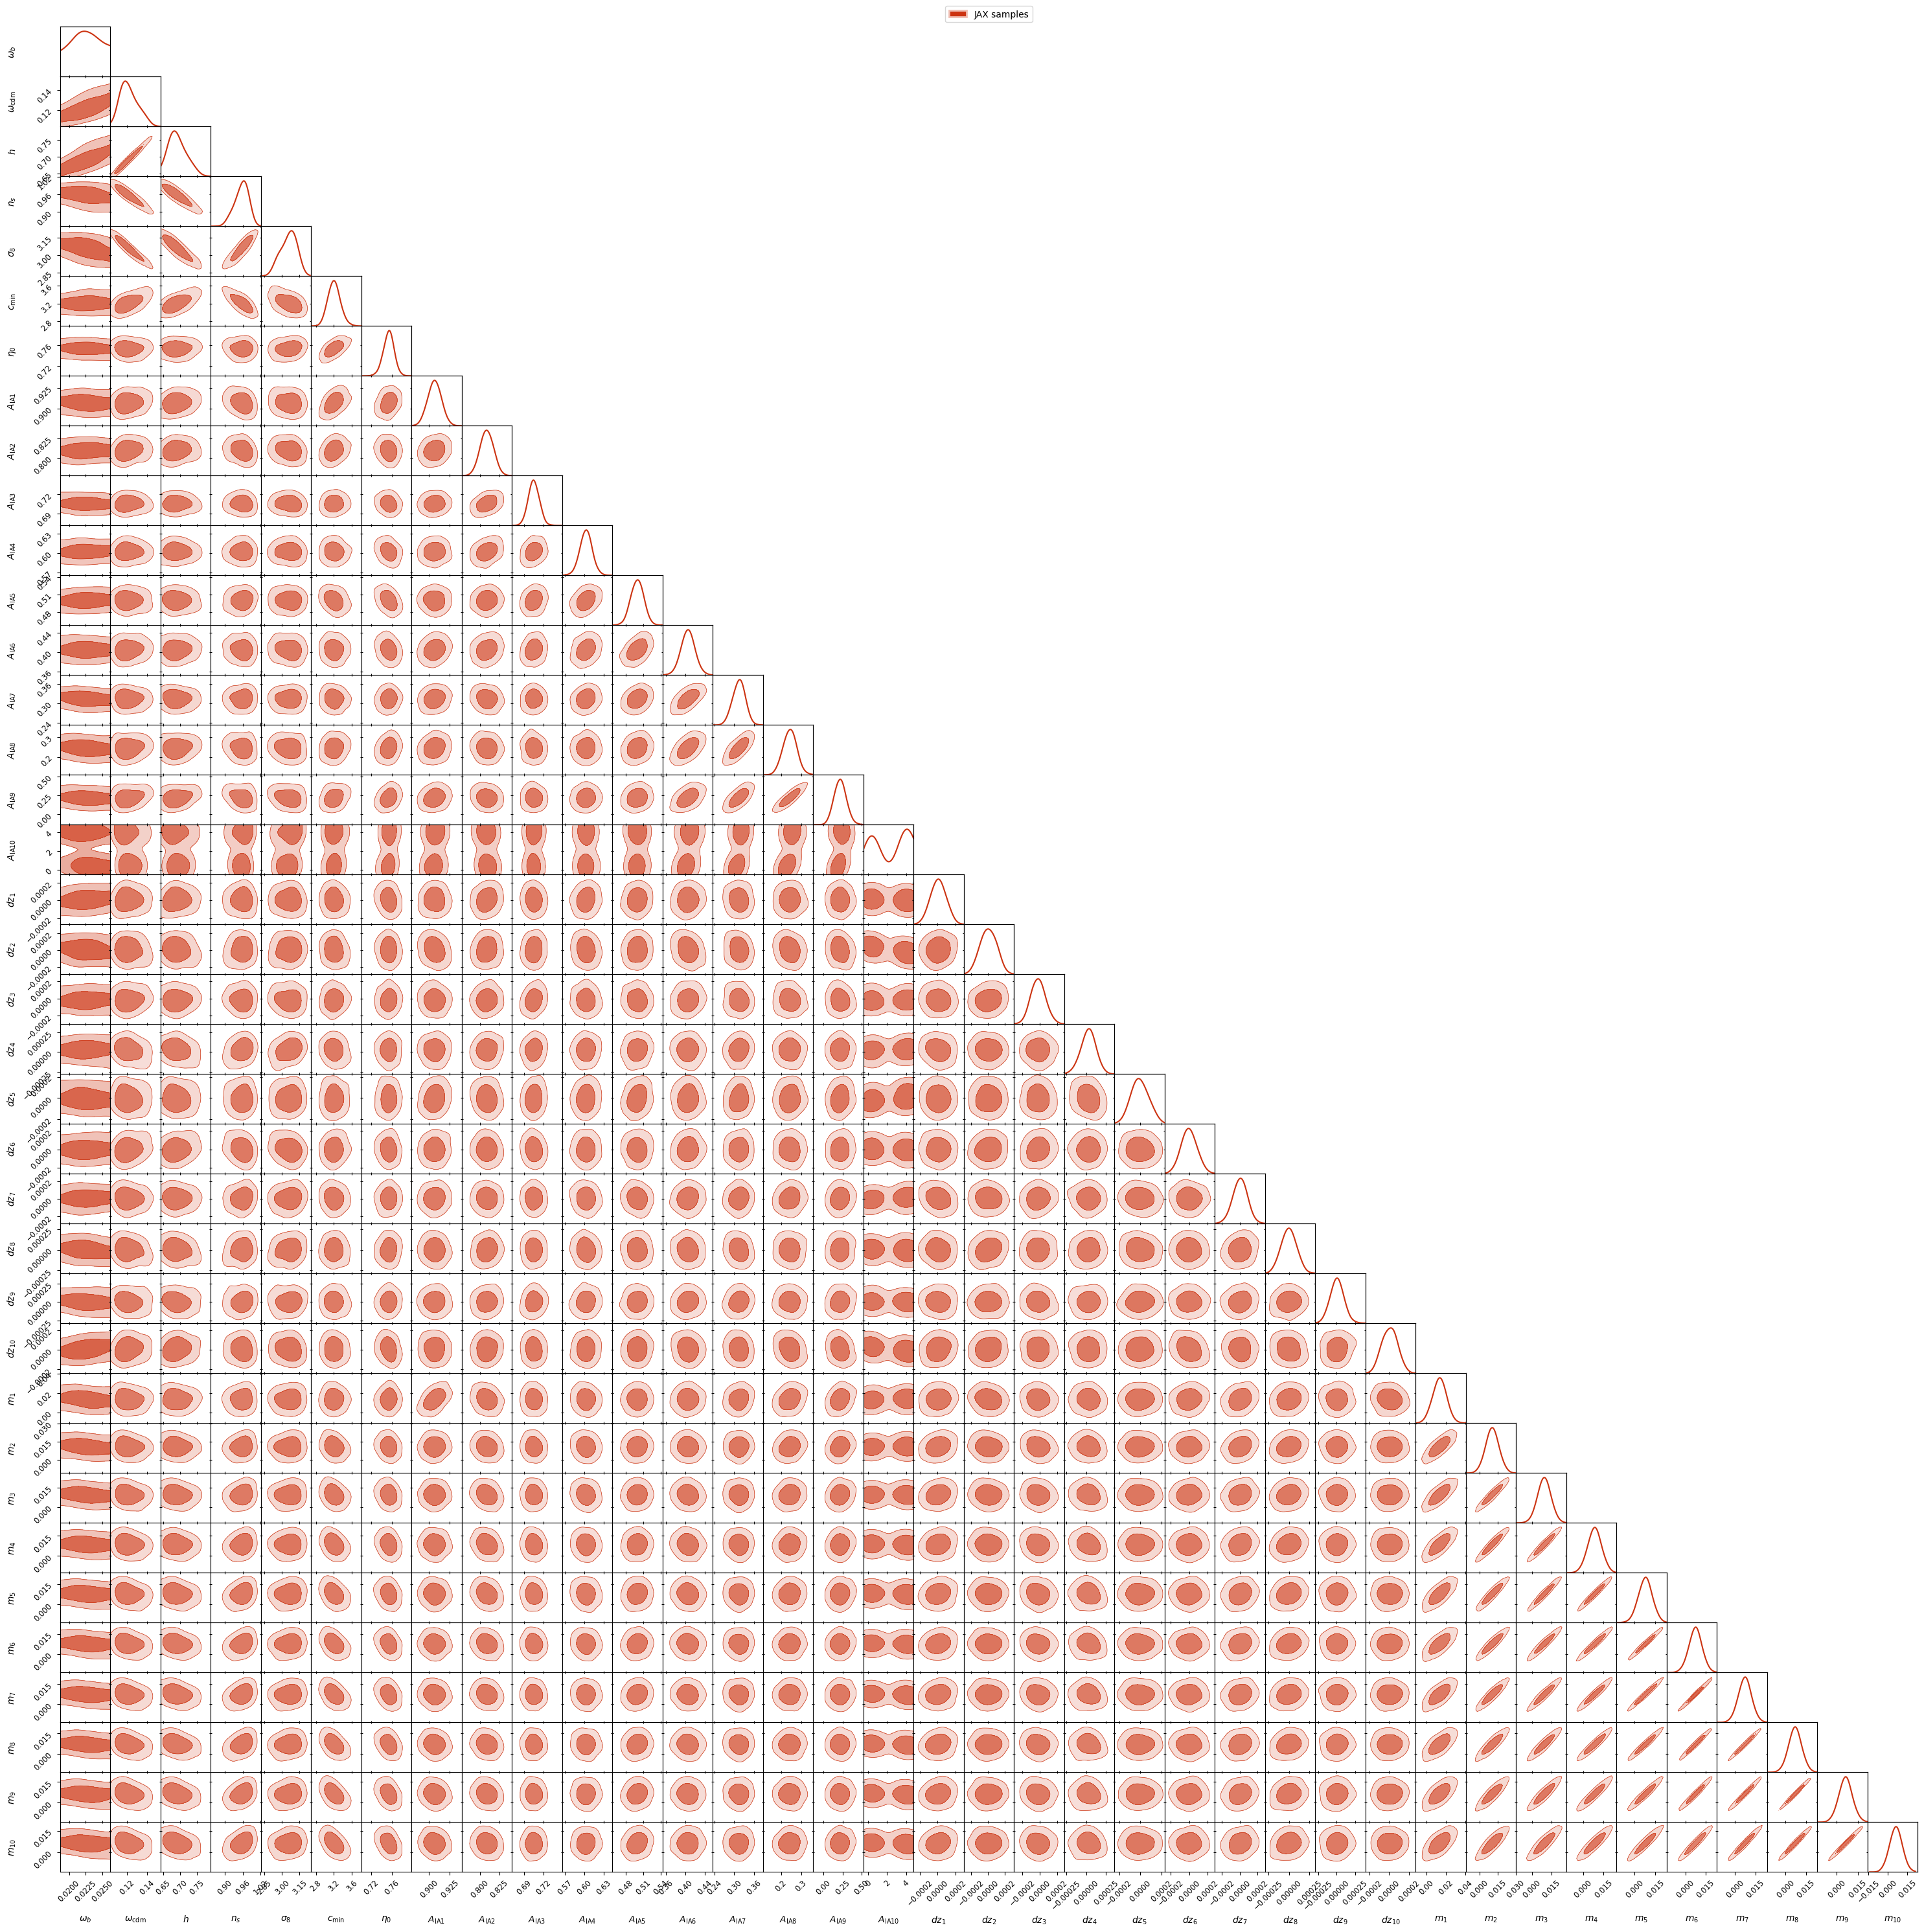
\includegraphics[width=\textwidth]{jaxSHEARfull.png}
    \caption{Full posterior constraints for the 39 parameters of the $w_0w_a$CDM Cosmic Shear model, obtained with GPU-NS. The plot reveals a bimodal structure in the nuisance parameter $A_{\text{IA},10}$, a feature that was not identified by the HMC sampler.}
    \label{shearfull}
\end{figure}

\end{document}